\documentclass[10pt,twocolumn,letterpaper]{article}

\usepackage{cvpr}
\usepackage{times}
\usepackage{epsfig}
\usepackage{graphicx}
\usepackage{amsmath}
\usepackage{amssymb}

% Include other packages here, before hyperref.

% If you comment hyperref and then uncomment it, you should delete
% egpaper.aux before re-running latex.  (Or just hit 'q' on the first latex
% run, let it finish, and you should be clear).
\usepackage[breaklinks=true,bookmarks=false]{hyperref}

\cvprfinalcopy % *** Uncomment this line for the final submission

\def\cvprPaperID{****} % *** Enter the CVPR Paper ID here
\def\httilde{\mbox{\tt\raisebox{-.5ex}{\symbol{126}}}}

% Pages are numbered in submission mode, and unnumbered in camera-ready
%\ifcvprfinal\pagestyle{empty}\fi
\setcounter{page}{1}
\begin{document}

%%%%%%%%% TITLE
\title{Variational Style Transfer}

\author{
Jan Schopohl
% For a paper whose authors are all at the same institution,
% omit the following lines up until the closing ``}''.
% Additional authors and addresses can be added with ``\and'',
% just like the second author.
% To save space, use either the email address or home page, not both
\and
Dominik Fuchsgruber
}

\maketitle
%\thispagestyle{empty}

%%%%%%%%% ABSTRACT
\begin{abstract}
   We propose a variational approach to neural style transfer, where the style of an artistic image is transferred to another. By using variational autoencoders to encode the style of an image, the latent style space is enforced to be smooth. This allows for better interpolation between different styles as well as sampling new unseen styles from the style space.
\end{abstract}

%%%%%%%%% BODY TEXT
\section{Introduction}

The task of artistic style transfer aims to extract the style of an (artistic) image and transfer it to the content of another picture. As has been shown in \cite{adain}, using an encoder-decoder architecture, where the decoder layers are conditioned on a style image using using \textit{Adaptive Instance Normalization} (AdaIn), can achieve visually pleasant results. Instead of using the same encoder module for style and content image, we follow Kotovenko et al. \cite{disentanglement} and make use of distinct encoders for content and style images.

Furthermore, we extend their approach by using a variational autoencoder architecture \cite{vae} to encode the style from an image. This enforces smoothness to the latent style space, which allows for better interpolation between different style embeddings. Additionally, we are able to draw samples from the latent style space, opening up a generative perspective to our approach.

%-------------------------------------------------------------------------
\section{Related Work}

Artistic style transfer was introduced by Gatys et al. in \cite{gatys}, who noticed that the style of an image is captured by the gram matrices of different feature maps of a VGG network. The heavy computational burdens of their approach led to the development of fully feed-forward architectures for style transfer. An autoencoder-based approach that is applicable to transfer arbitrary styles unseen by the model is introduced in \cite{adain}. They use \textit{Adaptive Instance Normalization}, which manipulates the instance-wise statistics of a content image before each decoder layer. This method was expanded upon by Kotovenko et al. \cite{disentanglement}, who proposed to incorporate two distinct encoders for content and style images.

\textit{Adaptive Instance Normalization} is also used to approach different problems, one of which being synthesizing photo-realistic video sequences of speech expressions for a particular individual \cite{talkingheads}. In our project, we heavily rely on the architecture of their encoder-decoder architecture. We extend the model by introducing U-Net \cite{unet} connections between the content encoder and the decoder.

The concept of encoding instances as distributions was first proposed in \cite{vae}. Sampling from those distributions during training enforces smoothness on the latent manifold.


\section{Our Approach}

Our model consists of three parts: Two distinct encoders for content and style images as well as a decoder that outputs stylizations.
\begin{itemize}
	\item The \textit{content encoder} takes a content image and applies a series of convolutions and poolings to it. The embeddings still retain a spatial extent, in contrast to just being flat vectors.
	\item The \textit{style encoder} is designed analogously to the content encoder, with the only difference being the use of adaptive pooling after the last convolution. Therefore, the style encoder yields a fixed-size embedding distribution by outputting the mean and variance of a normal distribution.
	\item The \textit{decoder} mirrors the design of the two encoders. It is preceded by several bottleneck layers, which do not change the resolution of the input image. Both the bottleneck layers as well as the upsamling convolutions are conditioned on the style embedding using \textit{Adaptive Instance Normalization}. Additionally, we use U-Net connections that connect the output of content encoder layers to the respective components of the decoder.
\end{itemize}
	
\begin{figure}
\centering
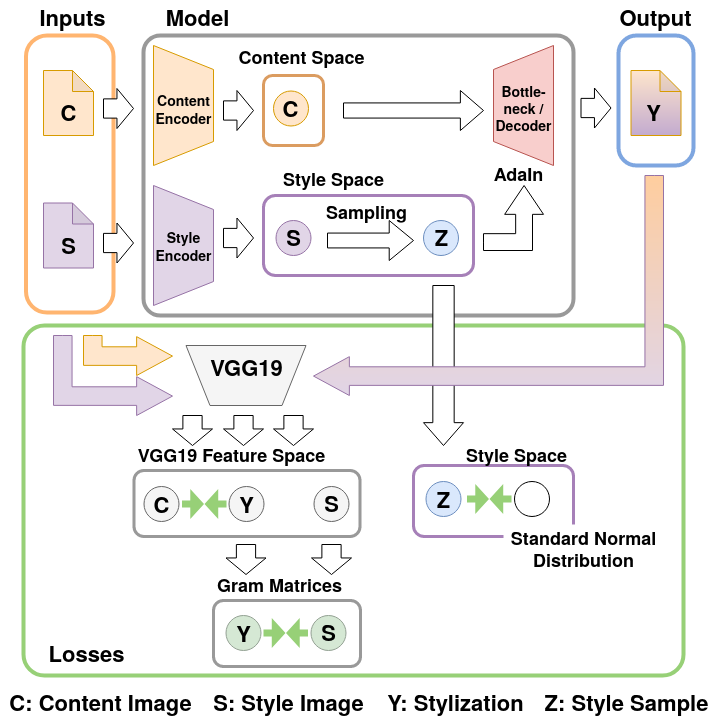
\includegraphics[width=0.9\linewidth]{pipeline_reduced_semi_verbose.png}
\caption{Visualization of the different components in our architecture as well as how the loss terms are implemented. Perceptual and style losses are computed in the VGG19 feature space.}
\label{fig:model}
\end{figure}
	
	
\subsection{Losses}

Our network is trained with respect to three different objectives. Apart from the variational prior on the latent space, those losses are computed in the features space of a pre-trained VGG19 network.
\begin{itemize}
	\item The content loss penalizes deviations of the stylizations regarding the content image and is implemented as a perceptual loss. That is, we consider the feature maps of the $relu_{4,2}$ layer of the VGG19 network.
	\item The style loss penalizes deviations from the style image by comparing the gram matrices of different VGG19 activation maps. We include layers up to $relu_{5,1}$ into the style loss term.
	\item The variational loss regularizes the latent space to resemble a standard normal distribution.
\end{itemize}

We assign different weights $\lambda$ to each summand of the content and style loss terms, as well as the variational loss.

\subsection{Datasets}

We use images from the \textit{Places365} dataset \cite{places365}, containing 1.8 million scenic photographs as content images. A subset of 100 images from the \textit{WikiArt} dataset is selected that exhibits a broad range of abstract and artistic styles. We explicitly exclude realistic paintings as they do not contribute to the learning of styles. For both datasets, images are downsampled and cropped to a resolution of 96x96 pixels.

\section{Results}

All the results we report are with respect to content images from a test dataset, while the style images are taken from the training data. This is due to the fact that we observed our model to be unable to generalize to unseen styles beyond just simple color transformations. Comparing with architectures of related work, we conjecture that this is due to the model complexity being to low. Because we lack the necessary GPU resources, we were however not able to verify this hypothesis.

\subsection{Variational and Non-Variational Autoencoders}
	
\begin{figure}
\centering
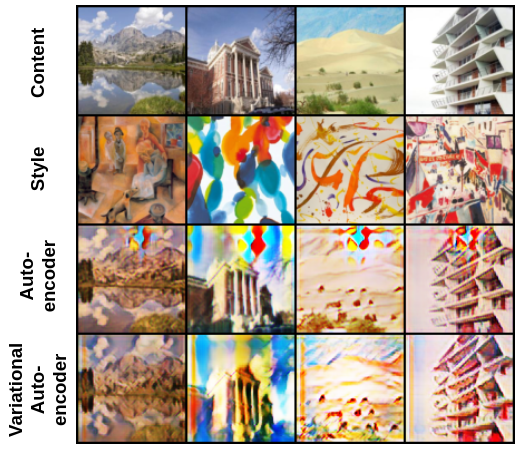
\includegraphics[width=0.9\linewidth]{ae_vs_vae.png}
\caption{Stylizations of Non-Variational Autoencoders and Variational Autoencoders}
\label{fig:ae_vae}
\end{figure}

First, we compare stylizations obtained by a model that uses a non-variational style encoder and compare it with the outputs of our proposed method. As can be seen in Figure \ref{fig:ae_vae}, we find that the introduction of sampling can prevent artifacts in the output image, as it also imposes regularization on the model itself. Furthermore, we find the overall quality of the variational approach to be visually more pleasing.

\subsection{Style Interpolation}

\begin{figure}
\centering
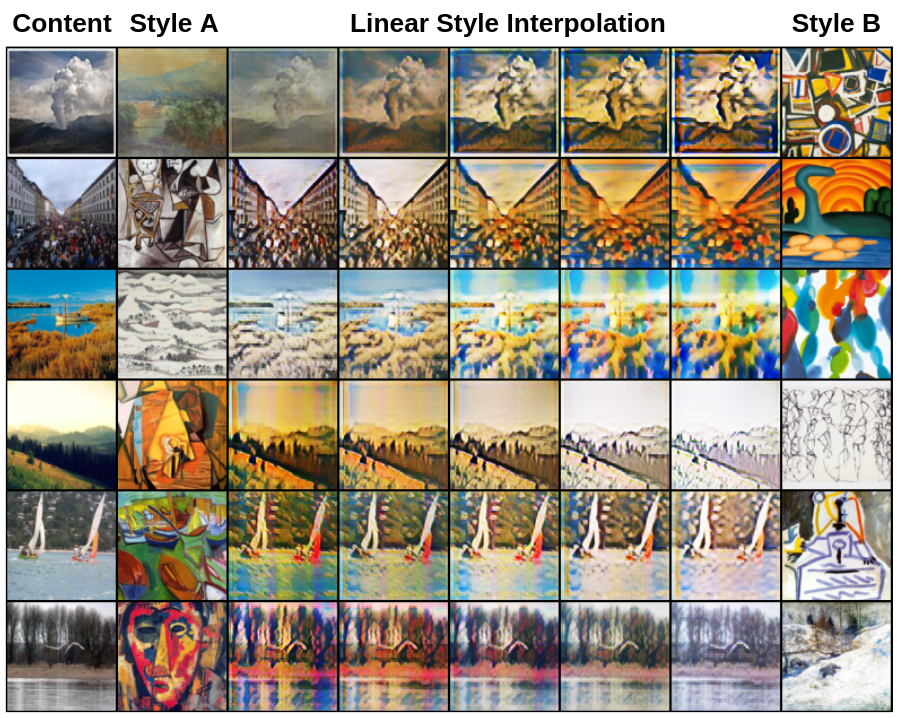
\includegraphics[width=0.9\linewidth]{interpolation.png}
\caption{Interpolating between two different styles}
\label{fig:interpolation}
\end{figure}

Figure \ref{fig:interpolation} shows that the smoothness of the latent space allows for a meaningful interpolation between two styles. That is in particular noteworthy, as our model has highly overfitted to 100 style images and nonetheless is able to provide appealing stylizations that mix two different style images. That means that even a model with no generalization capabilities at least yields a smooth latent style space containing the styles it was trained on.

\subsection{Style Sampling}

\begin{figure}
\centering
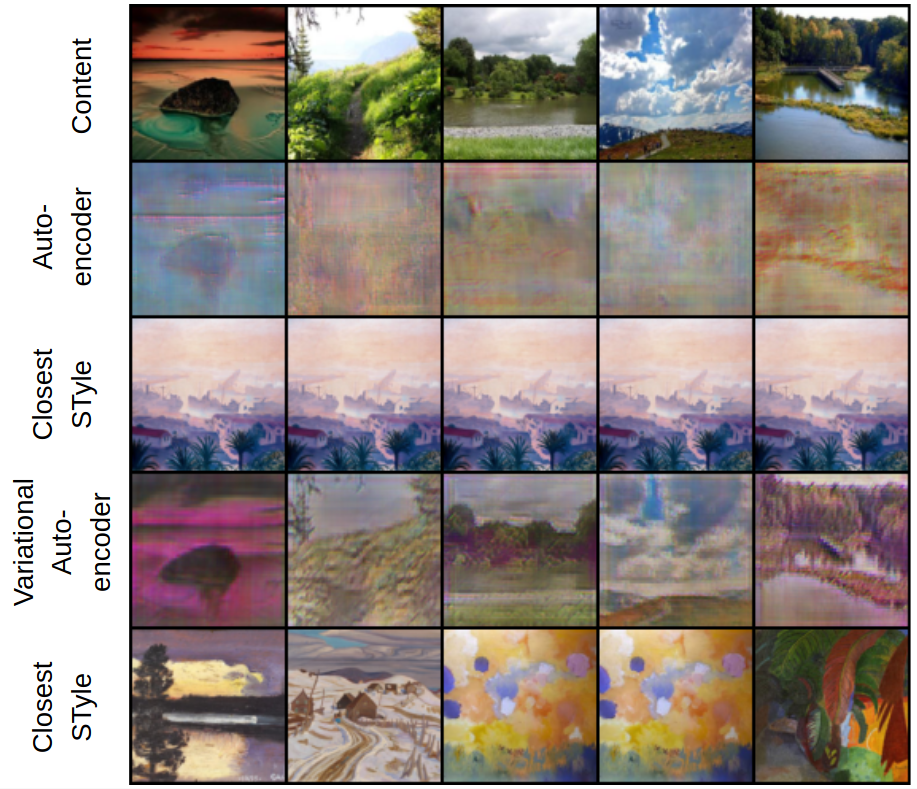
\includegraphics[width=0.9\linewidth]{sampling.png}
\caption{Sampling random styles and comparing with the style image most similar to the sample in style space}
\label{fig:sampling}
\end{figure}

Novel styles can be sampled by drawing random vectors from a standard normal distribution and conditioning the decoder on those. Figure \ref{fig:sampling} visualizes stylizations with randomly sampled style embeddings. It can be observed, that the variational approach visually outperforms the plain autoencoder architecture. In order to verify that the styles are indeed novel and unrelated to the style embeddings the model learned during training, we also show the style image that is most similar to the sampled style with respect to their latent representation. 

\subsection{Non-Expert Deception Rate}

We also conducted a survey among non-experts that were shown real artworks, stylizations provided by a non-variational autoencoder and outputs of our approach. Among five exemplars of each category the participants had to decide if an image they were presented was real or artificially generated. The images were shuffled before, and the participants were given a hard time-limit of five seconds to come up with a decision.

\begin{figure}
\centering
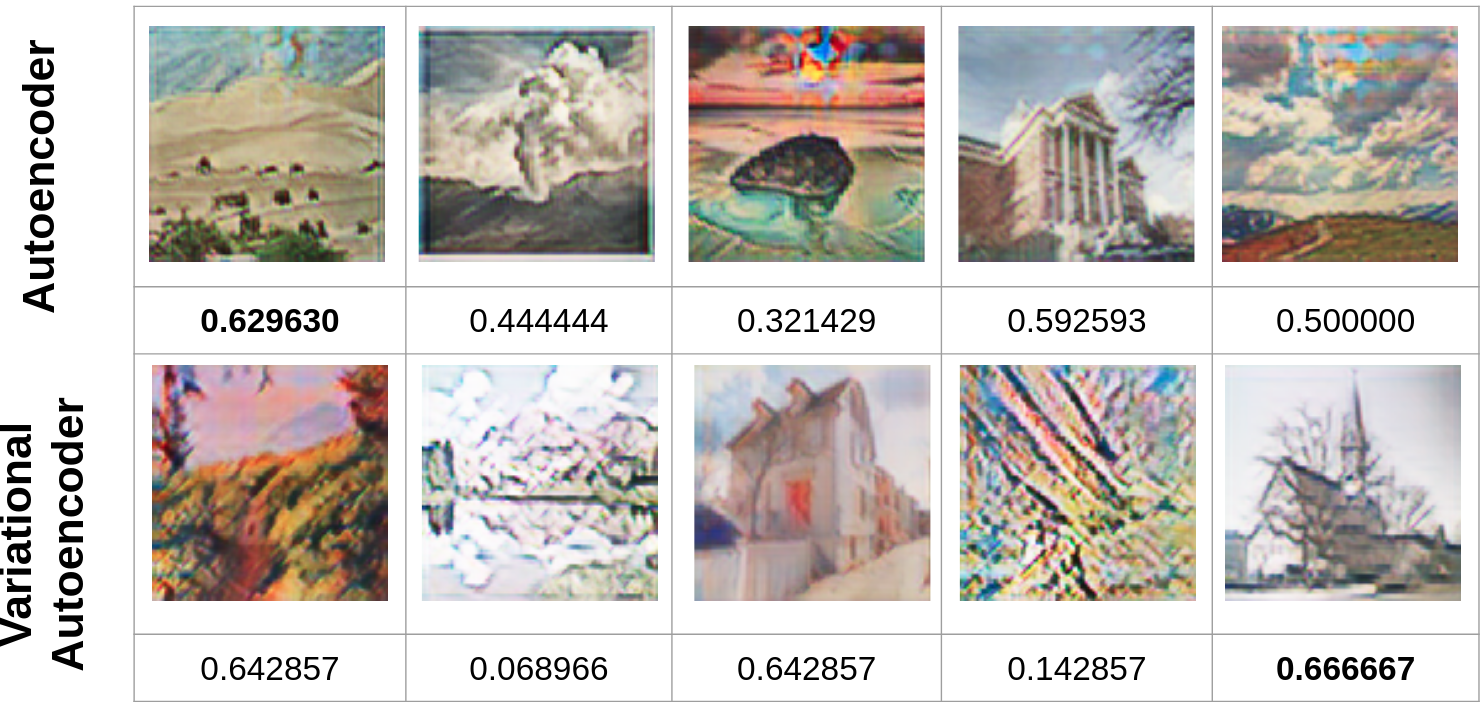
\includegraphics[width=0.9\linewidth]{survey.png}
\caption{Deception rate among non-experts for non-variational autoencoders and our approach.}
\label{fig:survey}
\end{figure}

Figure \ref{fig:survey} shows the results of our survey. While in general both approaches seem to perform similarly well, we observe that participants in general seemed to prefer non-abstract styles. Even though excluded from the figure, even in the case of real artworks low scores were recorded for abstract paintings. Nonetheless, two stylizations yielded by our approach outperform all five stylizations of the non-variational autoencoder.


\subsection{Variations in Style Space}

\begin{figure}
\centering
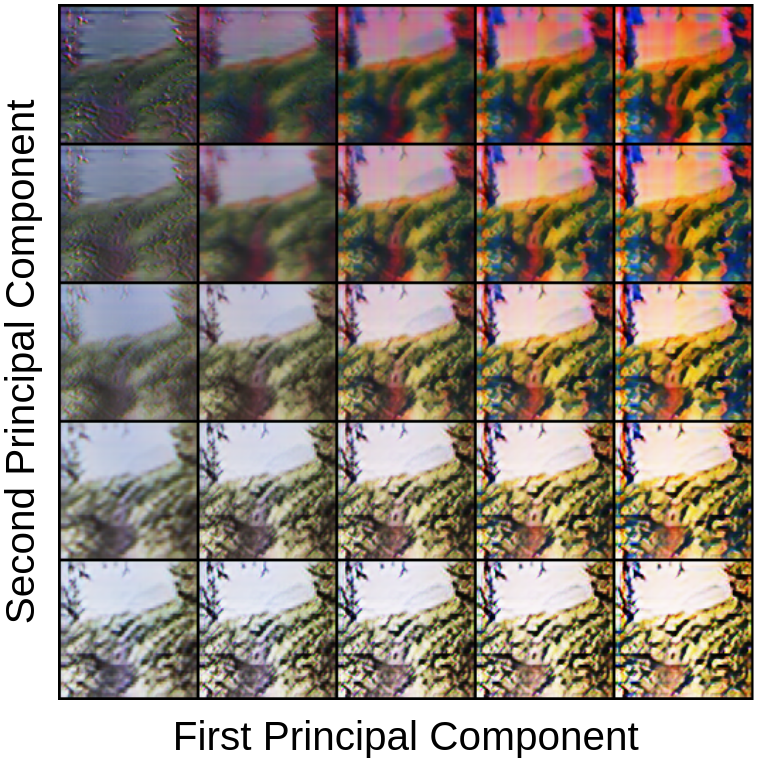
\includegraphics[width=0.8\linewidth]{pca.png}
\caption{Variations along first two principal components of the style space. The center image shows the unperturbed embedding.}
\label{fig:pca}
\end{figure}

To further verify smoothness of the style manifold, we perturb a style embedding along the first two principal components of the style space. Figure \ref{fig:pca} shows that those perturbations lead to smooth deviations in the model output.

\section{Conclusion and Future Work}

We propose an approach to artistic style transfer that embeds artworks into a smooth latent space making use of variational autoencoders. We show that this method allows for a smooth interpolation between different stylizations and also makes it possible to sample novel styles unseen by the model. Furthermore, introducing a variational prior on the style manifold imposes a regularization on the model that reduces artifacts in the output. 

Due to the lack of resources we were unable to train a model with generalization capabilities beyond simple color transformations. However, comparing our approach with related work, we conjecture that a more complex model might in fact to overcome this limitation. We leave it to future work to reevaluate our findings for a larger model.

{\small
\bibliographystyle{ieee_fullname}
\bibliography{egbib}
}

\end{document}
